\newpage
\section{評価実験}
\subsection{収縮率}
\subsubsection{内径3 mmの測定}
図\ref{fig:zA}に今回作製した内径3 mmの人工筋肉を示す.
測定方法は内径5 mmの測定と同様な方法で行った.
空圧を印加すると0.06Mpaが膨張の最大となった.
空圧印加前の長さは54 mm,空圧印加後の長さは49 mmで収縮率を求める式に代入すると
$$\frac{(49 \rm{mm})-(54 \rm{mm})}{49 \rm{mm}}\times 100\\$$
となり収縮率が9.3 \%となることが確認できた.
\begin{figure}[h]
    %
    \begin{minipage}{0.49\columnwidth}
      \vspace{4mm}
      \centering
      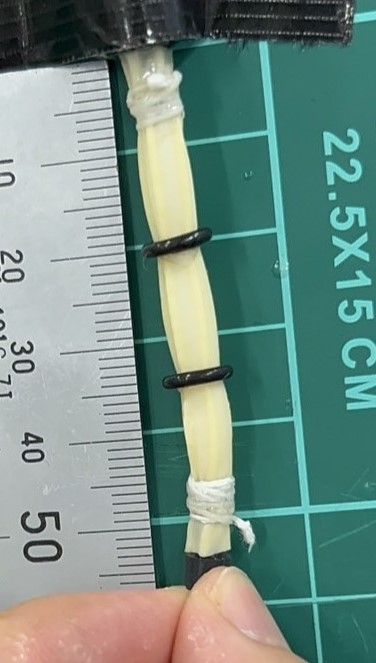
\includegraphics[scale=0.3]{pic/M.jpg}
    
      \subcaption{空圧印加前}

    \end{minipage}
    %
    \begin{minipage}{0.49\columnwidth}
      \vspace{4mm}
      \centering
      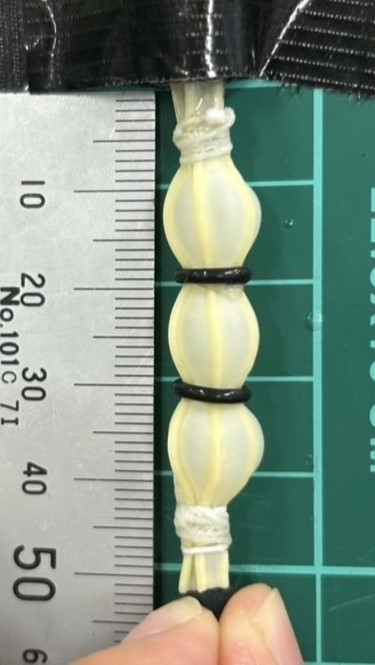
\includegraphics[scale=0.3]{pic/L.jpg}
      \subcaption{空圧印加後}
      
    \end{minipage}
    %
    \caption{内径3 mmの人工筋肉}
    \label{fig:zA}
  \end{figure}.
\subsection{発揮張力}
図\ref{fig:souti},\ref{fig:souti2}のような装置を使い発揮張力の測定を行った.またケブラーラインを通すために人工筋肉の先に図\ref{fig:new}を取り付けた.穴の直径は3 mmほど空いている.
測定に必要な物品は以下の通りである.
\begin{itemize}
  \item 作製した人工筋肉
  \item 万力
  \item S字フック
  \item 電子天秤 I 2000
\end{itemize}
測定手順を以下に示す.
\begin{enumerate}
  \item 作製した人工筋肉にケブラーラインを通す
  \item S字フックを取り付け電子天秤につなぐ
  \item 糸にテンションがかかる位置で万力に人工筋肉を固定する
  \item 電子天秤に電源をつけ,0点合わせをする
  \item 膨張の最大まで印加し,その時点での値を読み取る
\end{enumerate}
上記の手順で測定を行うと0.07Mpa印加した際に膨張が最大となり,その時点での電子天秤の値は138.4 gとなった図\ref{fig:138}.
このことから今回作製した人工筋肉が138.4 gまで持ち上げ可能な特性を有していることが確認できた.
\begin{figure}[h]
  %
  \begin{minipage}[b]{0.49\columnwidth}
    \vspace{4mm}
    \centering
    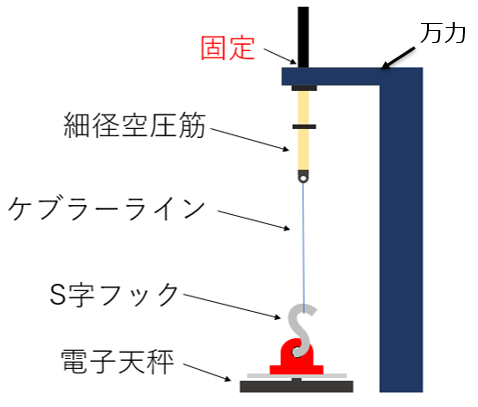
\includegraphics[scale=0.5]{pic/souti.PNG}
  
    \caption{測定装置のイメージ}
    \label{fig:souti}
  \end{minipage}
  %
  \begin{minipage}[b]{0.49\columnwidth}
    \vspace{8mm}
    \centering
    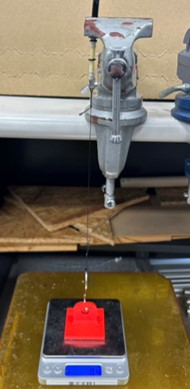
\includegraphics[scale=0.8]{pic/new.jpg}
    \caption{測定装置}
    \label{fig:souti2}
  \end{minipage}
  %
\end{figure}.
\begin{figure}[h]
  %
  \begin{minipage}{0.49\columnwidth}
    \vspace{4mm}
    \centering
    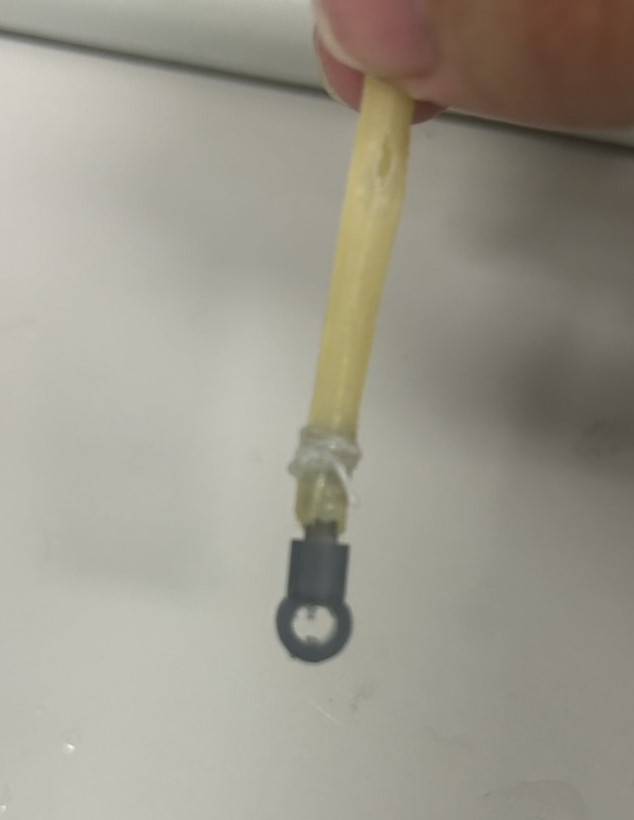
\includegraphics[scale=0.2]{pic/gg.jpg}
    \caption{開発した器具}
    \label{fig:new}
  \end{minipage}
  %
  \begin{minipage}{0.49\columnwidth}
    \vspace{4mm}
    \centering
    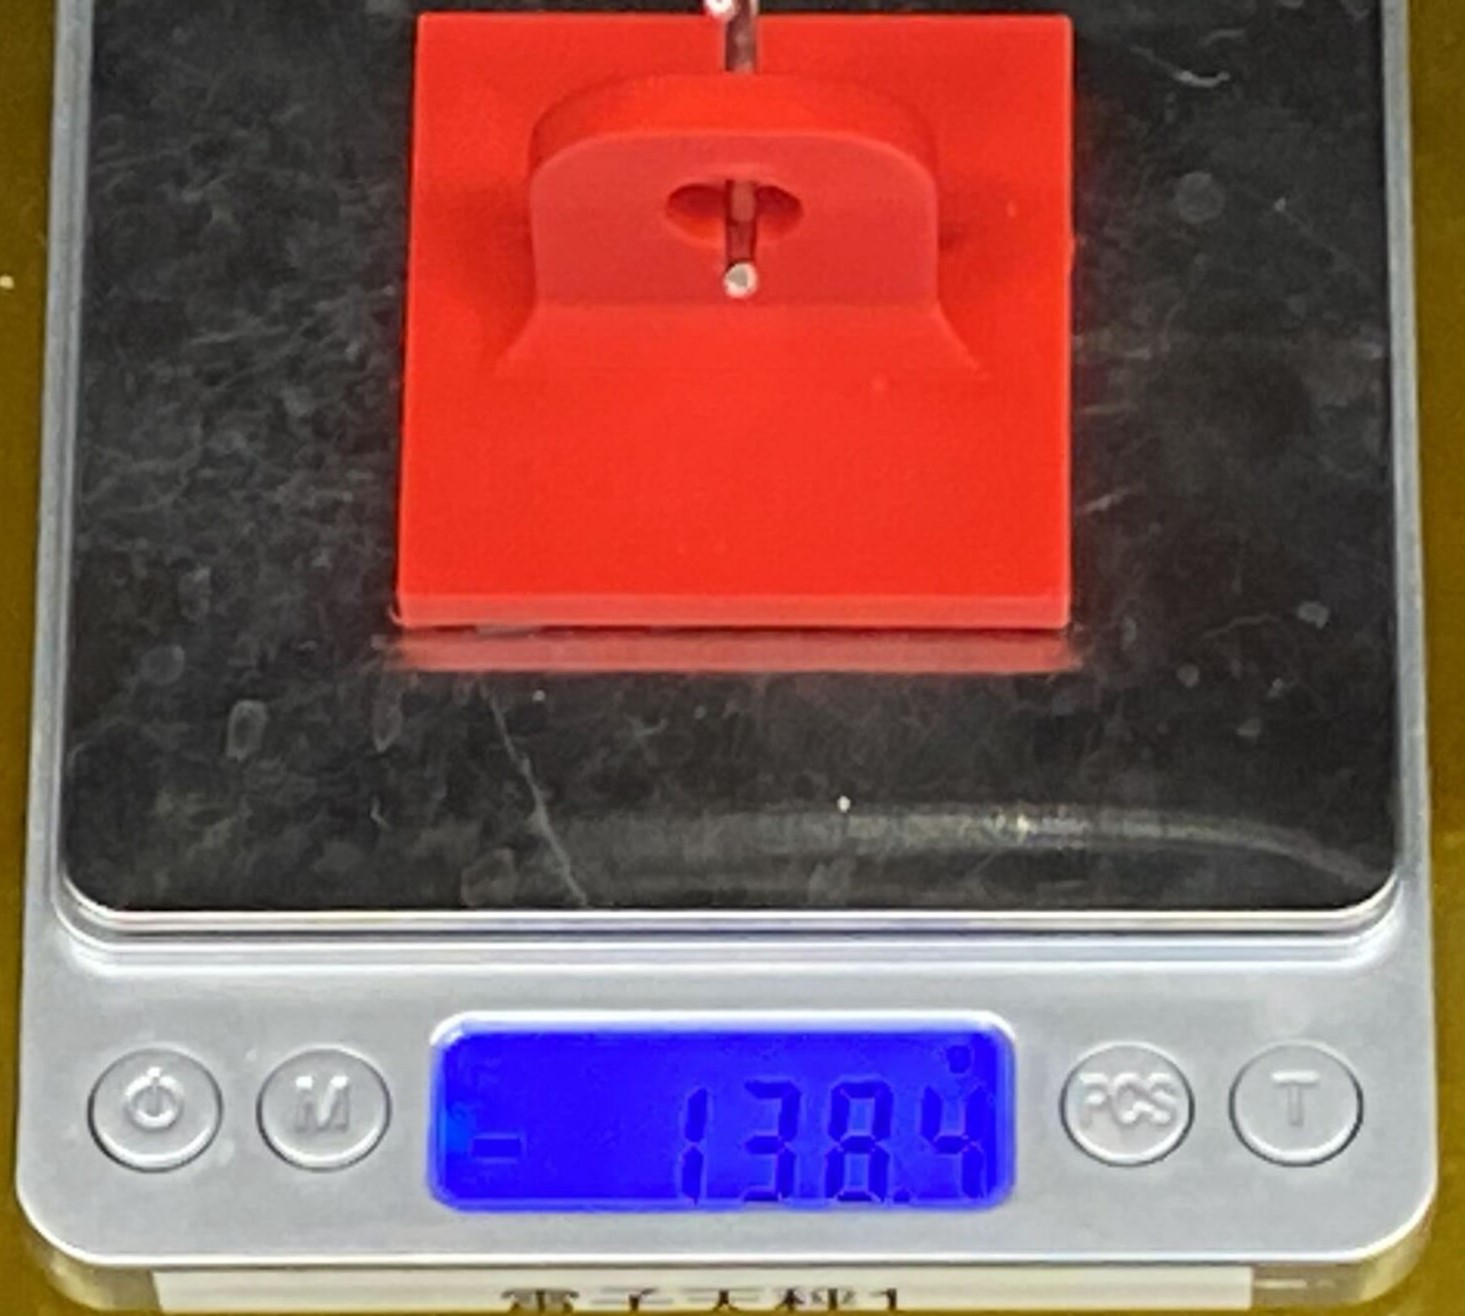
\includegraphics[scale=0.1]{pic/qqqq.jpg}
    \caption{電子天秤の値}
    \label{fig:138}
  \end{minipage}
  %
\end{figure}.

\newpage
\section{考察}
一般的な軸方向繊維強化型空気圧人工筋肉において
は,ゴムの膜厚は均一であり,その内部に縦糸が配置さ
れていることが一般的である.本研究でも,なるべくゴ
ム厚が均一になるよう,また糸がゴム膜の中に収まるよ
う作製方法を模索していった(図\ref{fig:mmm}\subref{fig:44}).
一般的な軸方向繊維強化型空気圧人工筋肉において
は,ゴムの膜厚は均一であり,その内部に縦糸が配置さ
れていることが一般的である.本研究でも,なるべくゴ
ム厚が均一になるよう,また糸がゴム膜の中に収まるよ
う作製方法を模索引き起こす結果となった.一方で,空圧筋として動作を
確認した作成方法5で作製した空圧筋(図\ref{fig:mmm}\subref{fig:44})においては,
糸はゴム膜の中央には配置されておらず,糸と糸
の間に薄いゴム膜を張るような構成となった.このこと
により,膨張がスムーズに行われ,空圧筋が高い柔軟性
を持ちながらも,必要な強度を確保することができた.
よって,今後より細径な空圧筋を開発する上ではゴム膜
の厚さと糸配置のバランスを取ることが重要であり,(図\ref{fig:mmm}\subref{fig:55})
のようにひだ状に作っていくことが有効であると
考えられる.
\begin{figure}[h]
  \centering
  % 上の4つの画像
  \begin{minipage}{0.49\textwidth}
      \centering
      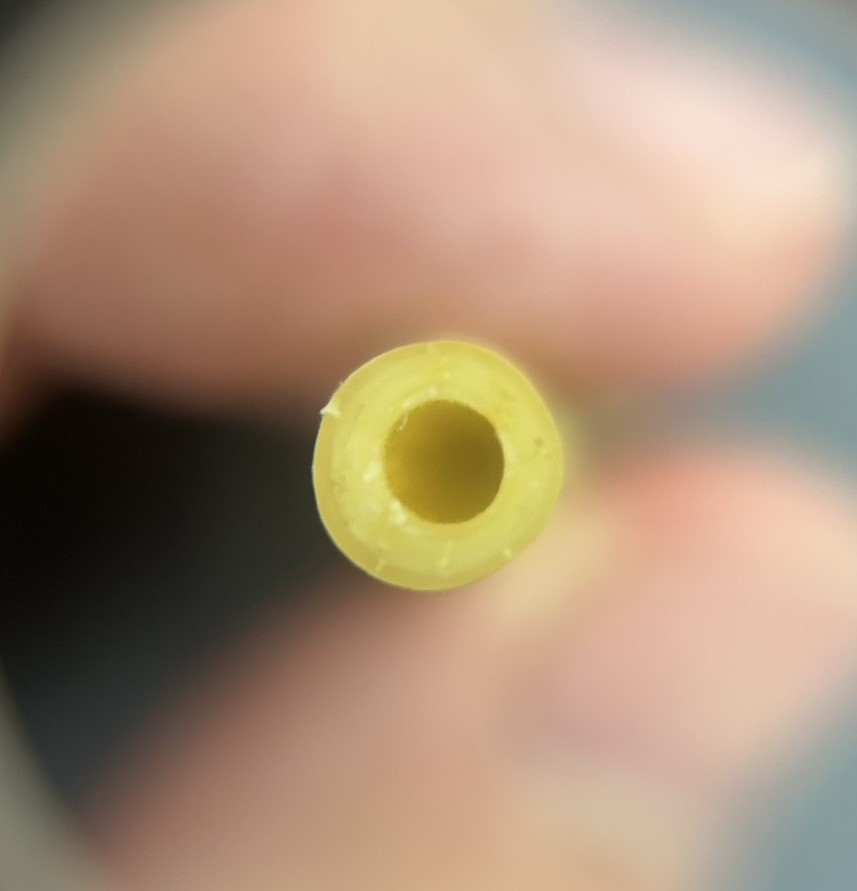
\includegraphics[scale=0.3]{pic/O.jpg}
      \subcaption{作成方法4}
      \label{fig:44}
  \end{minipage} \hfill
  \begin{minipage}{0.49\textwidth}
      \centering
      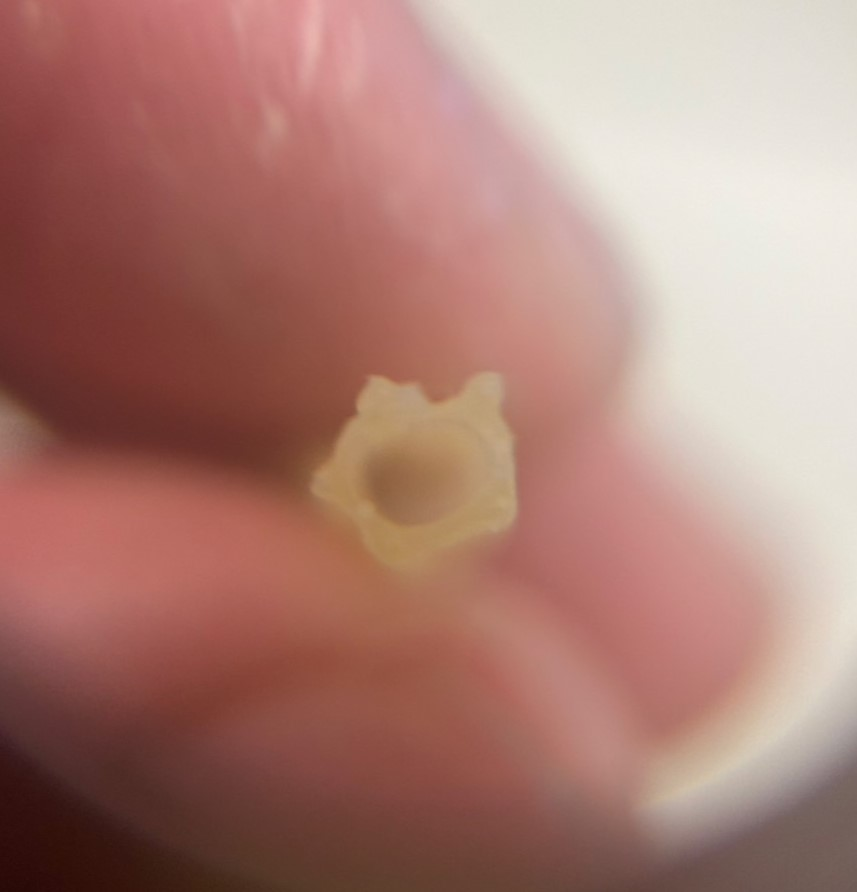
\includegraphics[scale=0.3]{pic/P.jpg}
      \subcaption{作成方法5}
      \label{fig:55}
  \end{minipage} 
  \caption{作成した細径空圧筋の断面}
  \label{fig:mmm}
\end{figure}

